\setlength{\columnsep}{3pt}
\begin{flushleft}
	\bigskip
	\begin{itemize}
		\item \textbf{A}ccess \textbf{C}ontrol \textbf{L}ists (ACL) allows a file to be \textbf{owned by several users 
			\& groups}, instead of single user \& group.
		\item Consider a directory named \textbf{project}. You need to provide permissions to this directory as below:
		\begin{itemize}
			\item User named \textbf{John} should have read, write and execute permission.
			\item User named \textbf{Jimmy} should have read and execute permission.
			\item Group named \textbf{managers} should have read, write and execute permission.
			\item Group named \textbf{testers} should have read and execute permission.
		\end{itemize}
		\bigskip
		This is possible by applying ACL rules.
		\begin{figure}[h!]
			\centering
			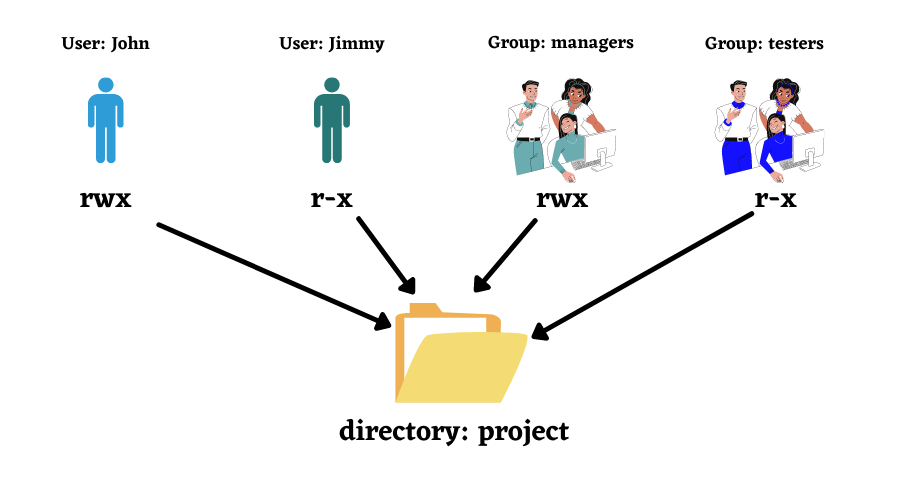
\includegraphics[scale=0.6]{content/chapter6/images/acl.png}
			\caption{ACL example}
			\label{fig:acl_example}
		\end{figure}

		
		
		
	\end{itemize}

	
\end{flushleft}

\newpage

